\newcommand{\comments}[1]{}
\documentclass[conference,a4letter]{IEEEtran}
\hyphenation{}
\usepackage{graphicx}
\usepackage{mathrsfs}
\usepackage{subfigure}
\usepackage{tabularx}
\usepackage{array}
\usepackage{algorithm}
\usepackage{amsmath}
\usepackage{epstopdf}
\usepackage{cite}
\usepackage[left=0.67in,right=0.67in,top=0.75in,bottom=1.05in]{geometry}


\begin{document}

\title{Manticore: a Distributed Overlay Networking Framework}

\author{\IEEEauthorblockN{
Fan Yang\IEEEauthorrefmark{1},
Jia-Liang Lu\IEEEauthorrefmark{1},
Clement Garnier\IEEEauthorrefmark{2},
Homere Faivre Saito\IEEEauthorrefmark{2},
Wei Shu\IEEEauthorrefmark{3},
and Min-You Wu\IEEEauthorrefmark{1}}
\IEEEauthorblockA{\IEEEauthorrefmark{1}Dept. of Computer Science \& Engineering, Shanghai Jiao Tong
University, Shanghai, China}
\IEEEauthorblockA{\IEEEauthorrefmark{2}Dept. of Telecommunications
Services  \&  Usages, INSA Lyon, Lyon, France}
\IEEEauthorblockA{\IEEEauthorrefmark{3}Dept. of Electrical \& Computer Engineering, University of New Mexico, USA}
Email: \{xcyangfan, jialiang.lu, mwu\}@sjtu.edu.cn,\{clement.garnier,homere.faivre\}@insa-lyon.fr,shu@ece.unm.edu
}


\maketitle



\begin{abstract}

The explosion of smart, wearable devices has introduced thousands of  smart objects to the market. While merely three or four systems are used, they are not connected smoothly to work collaboratively on a common goal. This paper presents Manticore, a cross-platform distributed overlay networking framework for smart devices. Based on Manticore, devices can discover the existence and capability of each other as well as establish publishing/subscribing service mutually. Manticore sets up an overlay networking layer and creates an abstractive view of devices and various on-board sensors. This approach shifts the focus from utilization of individual smart devices to the autonomous service discovery and establishment over self-organized networks. Manticore is composed of four elements: core, client, data-provider and end-point. All data transmission is carried by standard OSC data flow. Applications of Manticore in a number of interactive designs and musical syntheses have demonstrated agile utilization, extensibility and scalability.

\end{abstract}


\section{Introduction}
\label{sec:Introduction}
The recent advances in technology have provided us with numerous innovative ways to interact with others and devices in our daily life. The music and arts industry has not been left behind. Indeed, since the 1970s, synthesizers and electronic music have emerged over the classical music instruments, giving birth to many new styles of music. Nowadays, the accessibility and the rapid development of new devices enabling human to machine interaction such as wireless sensors have spawned a wide array of opportunities for new and more efficient music synthesis technologies and have introduced us to a  era of new media through the use of intelligent communicating devices.

The main objective of this work is to build a overlay networking framework to develop interactive concert platforms whilst using various types of communicating devices. That is to provide tools to manipulate and control different data inputs such as sensors transparently over a certain network infrastructure in order to create various outputs of an art performance such as music, lighting or even video projections.

A few key aspects have motivated the Manticore. First of all, the Manticore emerges as a desire to address the emerging field of ubiquitous computing and networking to the artistic real time context of live performances, and collaborative music synthesis. Although there has been extensive research in this field by leading institutes such as the Center for Computer Research in Music and Acoustics (CCRMA) at Stanford University or the Music Technology Department at McGill University, there yet have been consistent development of frameworks which could enable the musicians to make abstraction of network problematic when composing collaborative music over a network or when preparing live performances. Despite the few research initiatives in this field, such as Sense Stage from McGill \cite{SenseStage}, the wearable wireless sensor platform for interactive dance performances \cite{chu2006}, or  other sensor systems \cite{Ryan2003,Aylward2007,Torre2007,Todoroff2011} built for interactive performance, most of them are constricted to certain hardware architectures, such as the usage of pre-built wireless sensors.

Although some end-user products which have been on the market for the past few years such as  junXion \cite{STEIM} were in someway a solution to integrate any kind of sensor data, by proposing a wide array of usable human interface devices, such as but not limited to, joysticks, Arduino boards, and Wii motes. The recurring issue of adding a new sensor is unanswered, and furthermore,  the network capabilities were not exploited as much as they could be, or at least no proper foundation was laid to allow these kinds of improvements in the future. Such improvements could be for example the development of a multi-hop communication protocol that would enable nodes which are not able to communicate to exchange data through an intermediate node.


In addition to the inability of easily implementing extensions for new sensorial inputs, we have observed that there is a lack of tools that would bridge the gap between the network sensing and communication platform and the media programming platform which would be most familiar to the music programmer. Moreover, when this bridge exists, it is often between only one specific type of media programming platform such as Max/MSP \cite{maxmsp}. We thus seek to develop a framework, which would allow programmers to easily build upon it by adding new kinds of sensors, and new kinds of user-clients, such as Max/MSP, Processing\cite{processing}, etc.

The rest of the paper is organized as follows: Section \ref{sec:overview} gives a brief description of Manticore with both high-level and low-level architecture. In Section \ref{sec:implementation}, we introduce the implementation of Manticore followed by its working procedures and applications in Section \ref{sec:wpuc}. Section \ref{sec:Conclusion} discusses the potential of this work and future directions.


\section{Overview of Manticore}
\label{sec:overview}

In this part we will first give an overview of our global architecture, followed by the low level architecture of our software solution. We will then discuss about the network architecture adopted and the communication layers, agents that we have established and some use-cases.

\subsection{Global architecture (High-level architecture)}
\label{sec:highlevel}

The global architecture that is needed from musicians is a rather simple one which can easily be portrayed, like it has been done in Fig.\ref{fig:highlevel}. A wide spectrum of input data, which can be fed into the systems through different kinds of input systems such as  indoor localization platform, or human interface devices such as Wii Controllers, Leap Motion or Kinect. These inputs transfer data to a central system which processes it and outputs a desired sound, lighting, video or other devices.

\begin{figure}[htpb]
	\centering
			\includegraphics[width=3.1in]{eps/high.eps}
		\caption{Global architecture  of Manticore}
		\label{fig:highlevel}
\end{figure}

\subsection{Detailed architecture (Low-level architecture)}
\label{sec:lowlevel}

If we dive into the details of this architecture, we see that the input data, which comes from sensors that are sprawled over a well defined space, can be dispatched between several ``nodes". As pictured in Fig.\ref{fig:lowlevel}, we have decided to use Raspberry Pis\cite{pi} and the Cubiboard \cite{Cubie} as nodes since they're cheap, reliable and used to provide a convenient abstraction layer to the raw sensor data.

\begin{figure}[htpb]
	\centering
			\includegraphics[width=3.1in]{eps/low.eps}
		\caption{Detailed architecture  of Manticore}
		\label{fig:lowlevel}
\end{figure}

The created network can be seen as a wireless sensor network, where each devices (either the Raspberry or the Cubieboard) is a node of the network. We will hereby use the term ``node" in order to refer to the Raspberry Pis or the Cubieboards. Note that the term ``node" can also refer to any other ``computer device" that takes part in our framework.


\subsubsection{Network infrastructure}
\label{sec:networkinfra}

Modify the Figure -Pi +Cubi

The data which is to be transferred throughout our network is considered to be latency sensitive data, therefore the aspect of latency and jitter is of paramount importance when choosing our network infrastructure. Most of the current collaborative music applications (Some references are needed here, example of applications already existing) tend to run on cabled infrastructure for fear of the instability of wireless networks and high latency costs. However, we have chosen to approach this issue by proposing a solution that would be suitable for any kind of network technology, such as Wi-Fi local area, ad-hoc  and cabled local area networks.

While these solutions both present advantages and disadvantages, for practical purposes, such as the lack of cabling issues, the usage of a pre-existing Wi-Fi network has been used for the development of our project. However, it is not required to use Wi-Fi local  area networks, and this decision is completely up to the music programmer and his needs. // Try to make a focus on mobile crowdsensing ?

If he is composing a collaborative piece in a studio for music production, Wi-Fi can be considered as a viable solution. However, in the case of alive performance, many music engineers would prefer using a cabled approach to avoid connectivity and latency issues. In the next section, we will present our latency performances.

\subsubsection{Communication Layer}
\label{sec:communicationlayer}

In order not to rely on a specific software or implementation (e.g. Max/MSP is a proprietary software), we have decided to divide our framework into two main layers : a control plane and a data plane. This decision has mainly been made due to the influence of similar solutions in the field of telecommunications. 

// Like ZeroConf implementation ? Other examples ? Lake of references here. Make a small comparison with the reference that we will choose - Few lines. http://www.ijsr.net/archive/v4i2/SUB151428.pdf

\begin{figure}[htpb]
	\centering
			\includegraphics[width=3.4in]{eps/suc.eps}
		\caption{A simple use case}
		\label{fig:dataplane}
\end{figure}

Before explaining in a more detailed manner each of these two layers, we introduce a simple use case that will explain why such a division between control and data plane is  necessary for our network.

Consider that you are a musician/programmer, who wished to use sensor data from the sensors connected, for instance smartphones on the network of nodes. The local user client  provides an interface on which he/she can:
\begin{itemize}
  \item be aware of the current network capabilities, that is to say the nodes that are currently in the network, and the sensors, proposed by each of the nodes,
  \item request any number of these sensor data to be sent to the local client directly.
  \end{itemize}

Let us consider a network with two distant nodes, a remote, and a music workstation on which the user is. The use case can be described in the following steps:
\begin{enumerate}
\item A sensor is connected to a node (Cubieboard). This node detects the sensor, and advertises this new sensor through a communication agent we call the core, or Manticore.
\item Manticore on a distant workstation node is notified of this new sensor, and interacts with the Max/MSP local client to notify him of the network capability.
\item Having seen that a new sensor is available, the user, who is on the workstation, requests this sensor to his workstation��s Manticore.
\item The workstation��s Manticore will communicate with the Cubieboard's Manticore to request the resource, after checking that the resource is still available. During this phase, network information such as transfer port and IP address of the workstation will be communicated.
\item The Cubieboard's Manticore will check that the sensor is still available on its node, and will generate and execute a binary that sends the requested data to the provided IP address and port.
\item As a result the user will have a data stream sent to his workstation.
\end{enumerate}

Although, this use case seem to be fairly simple, we can easily think to extend and scale up this process with many more nodes (and of course sensors).

At the heart of the control plane, a core or as we call it Manticore, is a tiny program based on Node.js which is primarily dedicated to build an independent communication layer between all the nodes of the network. This communication layer establishes 3 communication channels :

\begin{itemize}
  \item Information Channel (InCh) on which each node is going to subscribe to each other, this channel is completely asynchronous. In the implementation, we use ZeroMQ\cite{Zeromq} abstraction library for sockets and a communication pattern of publisher/subscriber. Each node is a publisher and all others nodes on the network are aging to subscribe to it. Through this channel, each node will be notified whenever a distant node triggered an event (new device/sensor being plugged in). This channel enables all node to have an idea of the current network capabilities
  \item Main Channel (MaCh) implements a simple TCP client/server mechanism. The main channel (MaCh) implements the simplest request/reply mechanism. Nevertheless this mechanism can be achieved in 2 different ways:
\begin{itemize}
  \item a fully synchronous request/reply, when a node requests a resource, it waits for a direct answer (and thus blocks)
  \item an asynchronous request/reply, when a node issue an async request, it may expect (or not) a later reply but it does not block the current execution
\end{itemize}
  \item Local Channel (LoCh) dedicated for the local user clients communications. This communication, unlike the former two channels is based on an HTTP client/server communication pattern, in which the local user client is the HTTP client that
requests data through HTTP GET requests to Manticore, which houses an HTTP server.
\end{itemize}
The reason for which Manticore possesses these three above presented channels, is that we wanted to develop a core that would be able to exploit the network interface tools and be able to relay this data to the user client. Manticore is designed to be multi-platform.

The local client is designed to provide a user-friendly interface to the user within the data plane that will allow him/her to perform requests of resources/information over the network. This request is sent to the local core which will process it further to the recipient node (the node that has the requested sensor physically connected to it). The aim of this system is to develop a simple client through Max/MSP graphical programming language (external in Java or C++), although it can be imagined that this can be done for other media programming languages or frameworks for creative coding (i.e. Processing, openFrameworks, ...) allowing visual and many other aspects that can be combined with the music experience.

The data provider is the process within the data plane responsible for collecting raw data from sensors, formatting them into OSC packets and sending them to the proper workstation (that requested it). This data provider can simply be a pure data patch or even a complete driver (especially developed for a particular sensor). Sensed data are sent in OSC format which is widely used in the music field and is seen as the new MIDI allowing further possibilities, within UDP datagrams : these are real-time communications and we prefer to sacrifice the reliability to the latency and jitter.

\section{Application of Manticore}
\label{sec:wpuc}


In this section, we first introduce the working procedures of Manticore. After that, we demonstrate the flexibility and scalability of Manticore by showing some use cases.


\subsection{Working procedures}

Should 

At startup, a node advertises its presence by broadcasting a \_node.\_tcp service on Zeroconf. Doing so, other nodes can simply browse this service to dynamically discover its presence. We assume that all the nodes are on the same network segment (i.e in the same subnet). Thus we can infer that they can directly address other nodes using the recipient IP address. Each node provides different communication channels relying on a specific pattern : uni- or bidirectional, synchronous or asynchronous. The group messaging is achieved by the InCh implementing the publisher/subscriber network pattern. Hence, each node has 2 sockets : the publisher socket solely used to send information to all its subscribers and the subscriber socket solely used to receive information from all other nodes.  The point-to-point messaging is achieved by the MaCh implementing the request/reply network pattern. According to the situation, this request/reply can either be synchronous (an immediate reply is requested and thus will block the execution) or asynchronous (we expect a response but not urgently). To communicate with external processes, a HTTP server is embedded in each node
and can provide a web API, accepting GET request and serving JSON file or plain text status.

The distribution of the resource data is made using OSC packets on UDP datagrams. The main use case is a client that desire a resource provided on a specific node of the network. To achieve a proper delivery of the dynamic OSC data stream to this client, we use the information collected on both InCh and MaCh and execute the following procedure:
\begin{enumerate}
  \item A client issue a request on a local core to know the network status and resources available
  \item The server sends back a list of network nodes with its capabilities ( this list is known by the core through
  \begin{enumerate}
    \item Browsing of \_node.\_tcp service and
    \item Listening on any published event on InCh )
  \end{enumerate}

  \item The client issues a request on a resource, binds an UDP reception socket and waits for the core's response
  \item The local core knows which node to ask and issue in turn a synchronous request using MaCh. This is a synchronous request, meaning that it will waits for a reply.
  \item The recipient core handles this request, checks the availability of the requested resource, if so it sends a positive reply to the requester core. At the same time, it may generate a file and execute a program/driver that will send the data to the requester client.
  \item The local core receives the response, processes it and can now answer the client. A OSC stream over UDP must now be flowing between from the node with the requested to resource to the client
\end{enumerate}

\subsection{Use cases}

\subsubsection{General use case}
This use case is the simplest universal scenario that a user can encounter when using Manticore to perform a collaborative music synthesis or live performance composition over a network. In this use case the user who is on a Node B uses a client with an end user interface to poll the available nodes with available resources on the network. In fig.\ref{fig:uc1}, the user requests a resource from Node A using the user client on Node B. The requested resource data is sent by the Node A's data provider to the Node B's endpoint.

\begin{figure}[htpb]
	\centering
			\includegraphics[width=3.4in]{eps/guc.eps}
		\caption{General use case}
		\label{fig:uc1}
\end{figure}

\subsubsection{Multiple node scenario : 3 distinct nodes}
This use case is one where the user wishes to interact with several distant nodes. In this use case the user who is on a Node A uses a client with an end user interface to poll the available nodes with available resources on the network. In fig.\ref{fig:uc4}, the user requests a resource from Node B and Node C using the user client on Node A. The requested resource data is sent by the Node B and Node C's data provider to the Node A's endpoint. This scenario pictures 3 nodes, but theoretically, any number of nodes can request resources from any number of nodes. In this scenario, Node B could as well request data from Node A and Node C. In the same manner, Node C could also request resources to Node B and Node A. As a matter of fact, nodes can request resources to themselves.

\begin{figure}[htpb]
	\centering
			\includegraphics[width=3.4in]{eps/_uc3.eps}
		\caption{Three nodes scenario}
		\label{fig:uc4}
\end{figure}


\section{Set up configuration}
\label{sec:Set up configuration}

In this section, we will dive into the software configuration and implementation of our main communication agent for which we have coined the term Manticore, as well as the implementation of our end-user client on Max/MSP.

\subsection{Manticore}
Manticore's implementation mainly uses Node.js and a few different libraries for network service discovery, socket abstraction and manipulation. Node.js is a platform built on Chrome's Javascript runtime for building, scalable network applications. There are several reasons why we decided to use Node.js for our Core. First of all, Node.js has been, over the past two years, gaining popularity amongst developers, even for applications not concerning web programming. It is thus a runtime environment on which a large array of efficient libraries are available like mdns (for the node discovery), ZeroMQ (for the communication pattern and socket) etc. Furthermore, Node.js runs on javascript, thus does not need any compilation, and is available across different platforms, which is one of the key aspects which has been important to us during the development. Indeed, the main objective of our framework is to make musicians or music programmers jobs easier by avoiding to hassle with technical issues. Being able to have a framework working on different kinds of machines, and nodes is a must. Another very important aspect of Node.js is its event driven paradigm. This way of working enables Node.js to operates on a single thread, using non blocking I/O, allowing it to support a huge amount of transactions. For our project, an event-driven approach would ultimately be more efficient as transactions would be executed only when an event is triggered, avoiding to have to use excessive amounts of CPU time. For example, with the mdns library for Node.js, when a new network service is up, it triggers an event to notify that a new service is up. It avoids to have a loop to continuously check if a new service is up. In the end, Node.js was chosen because its developing community is extensive, hence the number of efficient usable libraries is high.

\subsection{Sensors}
\subsubsection{Type of sensors}
\begin{itemize}
\item MIDI Keyboard : how does it works, what is it, how do we integrate it to the manticore ?

\item Mobile devices such as tablets, smartphones (the main idea : Mobile crowdsensing) How does it work ? Examples of an event : a gig where the musician want some feedback from the crowd by using their smartphones / Multi platform iOS(phonegapp) + Android (native) / Implementation using websocket /Sending different kind of data
\end{itemize}


\subsection{End-user interface}

We have implement two end-user interfaces, that is to say one in the form of externals for the media programming language Max/MSP and another in the form of web interfaces, thus usable on any kind of platform.

\subsubsection{Max/MSP externals}
Max/MSP is a visual programming language for music and multimedia developed by a San Francisco based software company called Cycling 74. During its 20-year history, it has been used by composers, performers, software designers, researchers, and artists for creating recordings, performances, and installations. It has been favored by this community as it good for testing complex solutions, and very effective for prototyping and working with sensors.

From a developer's point of view, Max is a modular program, using shared libraries. It allows third-party development of new external objects called externals. The main functions of a Max/MSP external in Java are:
\begin{itemize}
  \item Communication through a HTTP connection with Manticore. This is done either when the user wants to get network information, or the user requests a resource.
  \item Creating a graphical interface according to the network information. This interface shows useful information for every node on the network, such as the sensors associated to it, network information such as IP address, associated port, hostname, and it also allows user to see the OSC syntax of the data that can potentially be sent by the sensor. Ultimately, this interface allows the user to choose the sensors he wishes to subscribe to.
  \item The subscription to a sensors creates and endpoint, that is to say a ``udpreceive" socket which allows the user to receive OSC data on a specific port from a specific sensor
\end{itemize}

\subsubsection{Web interface}
The web interface is a HTTP server running on the localhost, port 3000. It is a simple interface, which has the advantage of being accessible from a browser. It showcases the basic network information such as the nodes present on the network with their network information (IP address, hostname) and their associated sensors. This interface also enables the user to directly request a resource, and release it. Although this interface does not create endpoints, like the ``udpreceive" sockets in the Max/MSP client, they enable the user to use it like a universal client, which they can use with any other software.

\subsection{Performance experimentations}
What is the test environment? Requirement ?

\subsubsection{Performances and latency}
\begin{itemize}
 \item Latency when requesting a mobile from a pool of 20 sensors (graph + analysis)
 \item Latency when requesting an inertial sensor from a pool of 20 sensors (graph + analysis)
 \item Making 20 requests in the same time (analysis)
 \item (Latency when moving the phone ? Not that relevant ?)

\end{itemize}
To test the performance of the Manticore, we record the time for a new node joining the network under different number of nodes in the network. As shown in fig	.\ref{fig:data}, the average time of discovering, publishing/subscribing and finishing total procedures for a new node is increasing slowly as the growth of total nodes in the network, which demonstrates the scalability of Manticore.

\begin{figure}[htpb]
	\centering
			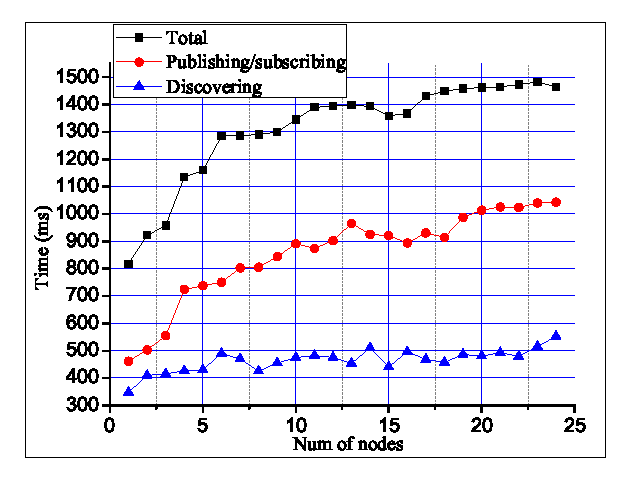
\includegraphics[width=3.1in]{eps/data.eps}
		\caption{Average time for discovering, publishing/subscribing and total procedures}
		\label{fig:data}
\end{figure}
\subsubsection{Comparison with existing projects}
Is there some existing projects ? Same architecture ? etc

\section{Conclusion}
\label{sec:Conclusion}
In this paper, we present Manticore, a new cross-platform  distributed overlay networking framework for smart devices. This framework is unique as it enables smart mobile devices to acquire the existence and capability information of each other, and establish publishing/subscribing service mutually. Thus, users can request resources distributed over the same network through this autonomous service discovery. Manticore allows musicians to use one of the most used softwares in the industry, namely Max/MSP. It also allows for incorporation of any kind of sensor which makes the application sustainable. Most important of all, this framework can become a powerful tool for musicians who want to create music or live performances over a local area network. These applications have demonstrated agile utilization, extensibility, scalability and robustness of Manticore.

\bibliographystyle{unsrt}
\bibliography{bib/indoorLoc}

\end{document}
